% !TeX root=main.tex
\chapter{
پیش‌بینی برهم‌کنش دارو-داروی با رویکرد سیتم توصیه‌گر یادگیری عمیق
}

در این فصل، ابتدا داده‌ها و ویژگی‌ها معرفی می‌شوند. سپس الگوریتم جدیدی مبتنی بر ۱) ادغام شباهت‌های دارویی و ۲) سیستم‌های توصیه‌گر یادگیری عمیق برای پیش‌بینی برهم‌کنش دارو - دارو در حالت جامع سه کلاسه ارائه می‌شود. الگوریتم مذکور
\lr{SNF-CNN}
نامیده می‌شود که مخفف
\lr{Predicting Comperhensive Drug - Drug Interaction via Similarity Network Fusion and Convolutional Neural Networks}
است. در این الگوریتم ابتدا روند آماده‌سازی داده‌ها توضیح داده می‌شود و سپس سیستم توصیه‌گری طراحی و بروی برهم‌کنش‌‌‌های افزاینده و کاهنده آموزش داده ‌می‌شود که جفت دارو‌‌های بدون برهم‌کنش را، با احتمال بالا تشخیص می‌دهد. در ادامه سیستم توصیه‌گر قبلی که مبتنی بر شبکه‌ی عصبی کانولوشن است، برروی داده‌‌‌های برهم‌کنش افزاینده و کاهنده و بدون برهم‌کنش (تشخیص داده‌شده در مرحله‌ی قبل) آموزش داده می‌شود. نتایج در روند اعتبارسنجی متقابل 10 برابری
\LTRfootnote{10-fold CV}
ثبت و در فصل چهار تحلیل می‌شود.

\section{داده‌ها و ویژگی‌ها}

در این پژوهش از مجموعه داده‌ای که در مقاله
\cite{Yu H2018}
ارائه شده است، استفاده می‌شود. این مجموعه شامل 568 داروی کوچک مولکول تایید شده است که هر دارو حداقل یک برهم‌کنش با دیگر دارو‌‌های مجموعه دارد. درمجموع برهم‌کنش‌‌‌های بین این ۵۶۸ دارو شامل 21351 برهم‌کنش است، که متشکل از 16757 برهم‌کنش افزاینده و 4594 برهم‌کنش کاهنده می‌باشد. 

علاوه‌براین، هر دارو با دو بردار ویژگی ۸۸1 بعدی ساختار شیمیایی
$F_{str}$
 از 
\lr{PubChem}\cite{Y. Wang2009}
 و 9149 بعدی عوارض جانبی خارج از برچسب
$F_{se}$
 از 
\lr{OFFSIDES}\cite{Tatonetti2012}
 نشان ‌داده می‌شود. برای جزئیات بیشتر به بخش 
\ref{ProbelmDefine}
 مراجعه کنید. 

داروها و برهم‌کنش‌ها تشکیل گراف می‌دهند. در این گراف گره‌ها دارو و یال‌ها برهم‌کنش هستند. جزئیات مجموعه‌ی داده‌‌‌های برهم‌کنش در جدول
\ref{dataDetail}
 ذکر شده‌است.
\begin{table}[h!]
\centering
\begin{tabular}{|c|c|c|c|c|c|c|c|}
\hline
خصوصیت & مقدار & درجه & مقدار & درجه‌ی
\lr{E-DDI}
  &  مقدار  &  درجه‌ی
\lr{D-DDI}
 & مقدار
\\
\hline
تعداد دارو 
&568 &
میانگین
& ۷۵/۱۸
& میانگین
&۵۹/۰۰
& میانگین
 & ۱۶/۱۸
\\
\hline
تعداد 
\lr{DDI}
&21351 &
میانه
& ۶۱/۵۰
&میانه
&۴۵/۰۰
&میانه
 & ۸/۰۰
\\
\hline

تعداد 
\lr{E-DDI}
 & 16757 &
بیشینه
& ۲۹۶
& بیشینه
&۲۳۰
&  بیشینه
 & ۲۰۶
\\
\hline
 
تعداد 
\lr{D-DDI}
 & 4594 &
 کمینه
& ۱
& کمینه
&0
& کمینه
 & ۰
\\
\hline
\end{tabular}
	\caption{
جزئیات مجموعه‌ی داده‌‌‌های برهم‌کنش
\cite{Yu H2018}
}
	\label{dataDetail}
\end{table}

\section{مدل‌سازی مسئله
\label{ProbelmDefine}} 

 
$D={\lbrace d_i \rbrace} , i=1,2,3,...,m$
را به‌عنوان مجموعه‌ای از
\lr{m}
داروی تایید شده دارای برهم‌کنش تعریف می‌کنیم. برهم‌کنش بین
\lr{m}
داروی تایید شده را به‌صورت یك ماتریس مجاورت متقارن
\LTRfootnote{Symmetric Adjacency Matrix }
$A_{m\times m}={\lbrace a_{ij} \rbrace}$
در نظر می‌گیریم كه
\lr{m}
تعداد داروها می‌باشد و
$a_{ij}$
هر درآیه از ماتریس
\lr{A}
است. برای مقادیر 
$a_{ij}$
دو دیدگاه متفاوت وجود دارد: 


الف) دیدگاه دوکلاسه 
\LTRfootnote{Binary Approach}:
$a_{ij}=1$
 اگر دارو‌‌های 
\lr{i}
ام و 
\lr{j}
ام تاثیر متقابل شناخته شده داشته باشند و درغیراینصورت
$a_{ij}=0$
. در این دیدگاه تاثیر‌‌های شناخته شده همگی در یك كلاس و با برچسب یک نمایش داده می‌شوند و حالت‌‌های عدم تاثیر و حالت‌‌های ناشناخته با برچسب صفر نشان داده می‌شوند. 

ب)دیدگاه سه‌کلاسه
\LTRfootnote{Triple Approach}:
$a_{ij}=1$
 اگر دارو‌‌های 
\lr{i}
ام و 
\lr{j}
ام تاثیر متقابل شناخته شده افزاینده داشته باشند و 
$a_{ij}=-1$
اگر دارو‌‌های 
\lr{i}
ام و 
\lr{j}
ام تاثیر متقابل شناخته شده کاهنده داشته باشند و در غیر اینصورت
$a_{ij}=0$
در این دیدگاه تاثیرات شناخته شده ،خود به دو كلاس با برچسب‌‌های متفاوت تقسیم می‌شوند و همچنان حالت‌‌های عدم تاثیر و حالت‌‌‌های ناشناخته با برچسب صفر نشان داده می‌شوند. 

دیدگاه استفاده شده در این پژوهش از نوع سه‌کلاسه است. 

علاوه‌براین، هر داروی 
$d_i$
در
\lr{D}
به‌ شکل بردار ویژگی
\LTRfootnote{Feature Vector} 
\lr{p}-
بعدی
$f_i = \left[  f_1, f_2, ... , f_k, ... , f_p \right]$
نمایش داده می‌شود که
$f_k = 1$
بیانگر مشاهده‌ی ساختار شیمیایی دارو یا وقوع عارضه‌جانبی خارج از برچسب، در
\lr{k}
امین بعد بردار است و درغیراینصورت  
$f_k = 0$
می‌باشد. از آنجا که هر دارو دارای دو بردار ویژگی ساختار شیمیایی و عوارض جانبی خارج از برچسب می‌باشد، دو ماتریس ویژگی
$F_{m\times p}$
تعریف می‌شود. به‌قسمی که
 $F_{str}$
ماتریس ویژگی ساختار شیمیایی و 
$F_{se}$
 ماتریس ویژگی عوارض جانبی خارج از برچسب هستند. به‌عنوان توضیح کوتاه، داروی شناخته شده/تایید شده به داروهای موجود در
\lr{D}
گفته می‌شود و داروی جدید دارویی است، که هیچ برهم‌کنش مشخصی  با هیچ‌یک از داروهای
\lr{D}
ندارد. در این پایان‌نامه روی داروهای جدید غربالگری انجام می‌دهیم و پیش‌بینی می‌کنیم چقدر احتمال دارد یک داروی جدید با یکی یا بیشتر از داروهای شناخته‌شده برهم‌کنش داشته باشد. 

\section*{مدل
\lr{SNF-CNN}}

در بخش‌های
\ref{PepareSNF}
 و 
\ref{RecomDesign}
 به‌ترتیب روند آماده‌سازی داده جهت ورودی دادن به مدل‌های یادگیری ماشین توضیح داده شده است. در ادامه روند انتخاب و اعمال مدل توصیه‌گر روی داده‌ها شرح داده می‌شود. همان‌طور که در بخش
\ref{PepareSNF}
 توضیح داده خواهد شد، روند استفاده از ویژگی‌ها و شباهت‌های دارویی به نحوی است که مستقل از نوع آن‌ها می‌باشد. لذا مدل و روال آماده‌سازی داده برروی ویژگی‌ها با شباهت‌های متنوع قابل اعمال و قابل تکرار است. همچنین اگر تعداد ویژگی‌ها بیش از یک نوع باشد با استفاده از روش 
\lr{SNF}،
 ادغام شده و برای ورودی به ماشین آماده می‌شود. این ویژگی خاص امکان استفاده‌ی مجدد روش ارائه‌شده را برای حالت‌ها و داده‌ها مختلف فراهم می‌کند. همچنین با توجه به این خصوصیت می‌توان مدل را برای مسائل مشابه درحوزه‌ی توصیه‌گرها مورد استفاده قرار داد.
  
\section{
آماده‌سازی داده
\label{PepareSNF}}

از آنجا که دارو‌‌های جدید گره‌‌‌های جدا شده در شبکه برهم‌کنش هستند، نمی‌توانیم برهم‌کنش احتمالی آنها را تنها با اطلاعات توپولوژیکی استنباط کنیم. بنابراین، اطلاعات اضافی آنها (به‌عنوان مثال ساختار شمیایی یا عوارض جانبی) مورد نیاز است، که از نظر یادگیری ماشین به آنها ویژگی دارویی گفته می‌شود. ابتدا ویژگی‌‌ها را مبتنی بر مدل خود آماده می‌کنیم و سپس یک مدل یادگیری عمیق از پیش‌بینی برهم‌کنش را آموزش می‌دهیم.

\subsection{
محاسبه‌ی ماتریس شباهت دارویی}
همان‌طور که در بخش
\ref{ProbelmDefine}
مشاهده شد، مقادیر ماتریس ویژگی‌ها گسسته‌اند و همچنین ابعاد ماتریس‌ها زیادند (ساختار شیمیایی ۸۸۱ بعد و عوارض‌جانبی خارج از برچسب ۹۱۴۹ بعد). از طرفی الگوریتم‌های یادگیری ماشین با داده‌های گسسته‌ی با ابعاد بالا، خوب کار نمی‌کنند و نتایج مطلوبی به‌دست نمی‌آورند. لذا در ابتدا با استفاده از روش کسینوس مشروح در بخش
\ref{simCal}
 ماتریس‌های شباهت دارویی مبتنی بر ساختار شیمیایی و عوارض‌جانبی خارج از برچسب محاسبه می‌شوند. این ماتریس‌ها به‌ترتیب 
$S_{str}$
و
$S_{se}$
هستند که ابعاد این دو ماتریس 
$m \times m$
است. هر درآیه از این ماتریس مقادیری بین صفر و یک دارد و هر
$S_{i,j}$
از ماتریس‌های شباهت، مقدار شباهت داروی
$d_i$
و
$d_j$ 
است.

\subsection{
ادغام ماتریس‌های شباهت دارویی}
در این مرحله از روش ترکیب شباهت شبکه‌ای که در بخش
\ref{SNF}
توضیح داده ‌شد، استفاده می‌شود. با استفاده از روش مذکور ماتریس‌‌‌های شباهت ساختار شیمیایی و عوارض‌جانبی خارج از برچسب داروها با یکدیگر ادغام شد. خروجی این ادغام ماتریس شباهت جدید
$S_{snf}$
است که ابعاد آن
$568 \times 568$
است و هر درآیه‌ی آن مقداری بین صفر و یک دارد. برای ترکیب شباهت شبکه‌ای از بسته‌ی
\lr{SNFPy}،
پیاده‌سازی شده در پایتون
\LTRfootnote{Python}
موجود در آدرس
\cite{SNFPy2020}،
استفاده شده ‌است.

\subsection{تشکیل ماتریس ورودی}

در این مرحله ماتریسی با ۱۱۳۹ ستون، شامل ستون‌هایی به شرح زیر تشکیل می‌شود:

۱) جفت داروها : نام داروی
\lr{i}
ام و نام داروی
\lr{j}
ام.

۲) نوع تاثیر : کاهنده (۱-)، افزاینده (۱+) و نامشخص (۰)

۳) بردار شباهت ۵۶۸تایی داروی
\lr{i}
ام از ماتریس
$S_{snf}$

۴) بردار شباهت ۵۶۸تایی داروی
\lr{j}
ام از ماتریس
$S_{snf}$

۵۶۸ دارو داریم و برهم‌کنش هر دارو با خودش بی‌معنی‌است. از طرفی جفت داروهای 
$(d_i, d_j)$
و 
$(d_j, d_i)$
دوگان هم بوده و حضور هردوی آن‌ها در داده موجب افزایش داده‌های آموزش می‌شود که متعاقبا توان ماشین را در پیش‌بینی بهتر افزایش می‌دهد. درنتیجه ماتریس حاصل 322056 نمونه یا ردیف داده دارد. باتوجه به توضیحات ارائه‌شده، ماتریس 
$B$
با ابعاد 
$322056 \times 1139$،
جهت ورودی دادن به ماشین توصیه‌گر، تشکیل می‌شود.


\section{
طراحی سیستم توصیه‌گر
\label{RecomDesign}}

در مراحل قبل داده برای ورود به هر ماشین یادگیرنده از جمله ماشین‌های یادگیری عمیق آماده شد. اما قبل از ارائه‌ی مدل و ورود داده به ماشین باید یک نکته‌ی مهم را در نظر گرفت. همان‌طور که در بیان مسئله ذکر شد، چه در این تحقیق و چه در دیگر تحقیقات، داده‌های مثبت یک یا منفی یک برچسب‌های مشخص و معینی هستند. درحالی که برچسب صفر به هیچ عنوان به‌معنی عدم وجود برهم‌کنش در بین یک جفت دارو نیست، بلکه بیان می‌کند که برای این جفت دارو هنوز برهم‌کنشی یافت نشده ‌است. در ادامه روشی برای تشخیص جفت داروهای بدون برهم‌کنش ارائه می‌دهیم. سپس از این جفت داروها به عنوان داده‌هایی با برچسب صفر در آموزش بعدی استفاده می‌شود.

\subsection{روند انتخاب و آموزش مدل روی برهم‌کنش‌های شناخته‌شده}

برای حل این مسئله نیاز است مدلی ارائه شود که عدم برهم‌کنش را با دقت و اطمینان خوبی تشخیص دهد. داده‌ها و تحقیقات قبلی از داده‌های دوکلاسه استفاده می‌کردند که دراصل تنها دسته‌ی مثبت (وجود برهم‌کنش) قابل اعتماد است و نمی‌توان به دسته‌ی منفی (عدم وجود برهم‌کنش) اعتماد کرد. دراینصورت ارائه‌ی مدل با هدف تشخیص صفرهای واقعی‌تر با استفاده از داده‌های دوکلاسه امری سخت و کمتر قابل اعتماد است. از طرفی داده‌های سه‌کلاسه این نوید را می‌دهند که با افزایش دسته‌ و تقسیم بندی انواع برهم‌کنش، مشخصات عدم بر‌هم‌کنش به شکل بهتری توسط مدل‌ها بازنمایی شود.

باتوجه به توضیحات داده‌شده و با وجود استفاده از داده‌های سه‌کلاسه این تحقیق سعی می‌کند ابتدا مدلی مبتنی بر یادگیری عمیق ارائه دهد که عدم برهم‌کنش احتمالی جفت داروها را پیش‌بینی کند. بدیهی است، دقت بالا در تشخیص این صفرها می‌تواند در ارائه‌ی مدل سه‌کلاسه دقیق‌تر و قابل اعتمادتر کمک شایانی کند.

\subsubsection{روند اعتبارسنجی جهت انتخاب مدل
\label{Model_selection_CV}}
سطرهایی از ماتریس
\lr{B}
که شامل برهم‌کنش‌‌‌های مثبت یک و منفی یک هستند، جدا می‌شود. ماتریس جدید شامل 42702 جفت دارو با تاثیر کاهنده و افزاینده است. این داده برای آموزش و یافتن مدلی مناسب‌تر استفاده شد تا از بین تعداد زیادی از مدل‌ها با ساختارهای شبکه‌ای مختلف مدل قوی‌تری پیدا و استفاده شود. مدل نهایی شبکه‌ی عصبی عمیقی بود که از لایه‌های کانولوشن و تماما متصل بهره می‌برد.

ویژگی‌های همه برهم‌کنش‌ها (مثبت یک و منفی یک) شامل 1136 ویژگی است. در ابتدا این ویژگی‌ها را به 10 دسته مساوی تقسیم می‌کنیم. سپس در یک حلقه 10 تایی هر بار، یک دسته را به‌عنوان مجموعه ارزیابی و ۹ دسته دیگر را به عنوان مجموعه ‌داده آموزش در نظر می‌گیریم.

مدل‌های مختلفی را انتخاب کرده و در روند اعتبارسنجی مذکور با ۹۰ درصد داده‌ها، مدل را آموزش می‌دهیم. سپس بر روی ۱۰ درصد باقیمانده داده‌ها، ارزیابی مدل را انجام می‌دهیم. در روند جداسازی جفت داروهای دوگان درنظر گرفته شده است. از آنجا که جفت داروهای
$(d_i, d_j)$
و
$(d_j, d_i)$
از نظر زیستی فرقی با هم ندارند پس در جداسازی داده‌ی آموزش و ارزیابی همواره یک جفت دارو و دوگان آن لزوما در یک گروه یکسان قرار می‌گیرند. این امر از شبهه‌ی تقلب ماشین جلوگیری می‌کند.
 
در روند انتخاب مدل، از مدل‌های یادگیری ماشین کلاسیک نظیر جنگل تصادفی
\LTRfootnote{Random Forest}،
ماشین بردار پشتیبان
\LTRfootnote{Support Vector Machine(SVM)}، 
برازش بخت
\LTRfootnote{Logistic Regression}،
شبکه‌ی پرسپترون چند لایه
\LTRfootnote{Multilayer Perceptron}،
شبکه‌ی حافظه طولانی کوتاه مدت
\LTRfootnote{Long Short-Term Memory(LSTM)}، 
شبکه‌ی عصبی ‌کانولوشن یک بعدی و دو بعدی، شبکه عصبی مصنوعی
\LTRfootnote{Artificial Neural Network}،
خودرمزنگار و ترکیبی از آنها استفاده کردیم.


 \subsubsection{ارائه‌ی مدل انتخابی (شبکه عصبی کانولوشن)
 \label{selected_model}}

\begin{figure}[!h]
	\centering
	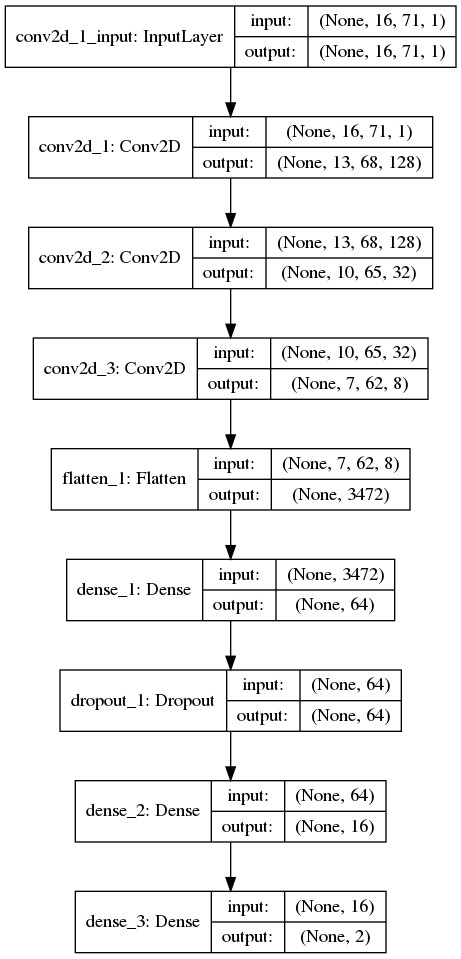
\includegraphics[scale=0.63]{section3/model.jpg}
	\caption{
نحوه‌ی چینش لایه‌های شبکه عصبی تشخیص صفرهای احتمالی}
	\label{CNNModel}
\end{figure}

بعد از آزمودن ساختارهای مختلف، شبکه‌ی عصبی عمیق مورد استفاده نهایی را همانند ساختار شکل
\ref{CNNModel}
مدل‌سازی کردیم. این شبکه دارای سه لایه کانولوشن دو بعدی و در امتداد آن سه لایه‌ی تماما متصل کانولوشن می‌باشد. لایه‌ی آخر دو خروجی برای پیش‌بینی تاثیر کاهنده و یا افزاینده دارد. لایه‌های‌ کانولوشن از فیلترهای مربعی با ابعاد ۴ و گام
\LTRfootnote{Stride}
۱ استفاده می‌کنند. همچنین هر لایه‌ی کانولوشن دارای یک تابع فعال‌سازی
\LTRfootnote{Activation Function}
\lr{Relu}
است. تعداد فیلترهای کانولوشن به ترتیب ۱۲۸، ۳۲ و ۸ می‌باشد. لایه‌های تماما متصل به‌ترتیب ۶۴، ۱۶ و ۲ گره دارند، دو لایه‌ی اول دارای فعال‌ساز
\lr{Relu}
بوده و لایه‌ی آخر با ۲ گره دارای فعال‌ساز 
\lr{Sigmoid}
می‌باشد. لایه‌های کانولوشن با استفاده از لایه‌ی هموارکننده
\LTRfootnote{Flatten}
به لایه‌های تماما متصل مرتبط می‌شود. وظیفه‌ی این لایه تغییر شکل مستطیلی دو بعدی به حالت برداری یک بعدی است. خروجی این لایه ورودی لایه‌ی اول تماما متصل می‌باشد. همچنین بین لایه‌های تماما متصل ۶۴ و ۱۶ گره‌ای از یک لایه‌ی
\lr{Dropout}
با مقدار دور ریخت ۰/۲ استفاده می‌شود.  مقدار ۰/۲ بیان می‌کند که شبکه در این لایه بصورت تصادفی بیست درصد ویژگی‌ها را درنظر نمی‌گیرد. این لایه بدین منظور استفاده می‌شود که از بیش‌برازش
\LTRfootnote{Overfit}
مدل جلوگیری کند و مدل را وادار می‌کند تا تعداد ویژگی‌های بیشتر و با اعتماد بالاتری را جهت پیش‌بینی استخراج و مورد استفاده قرار دهد و درصورت حذف تعدادی از آنها توان پیش‌بینی الگوریتم افت نکند و متکی به چند ویژگی خاص نباشد.
 
در بررسی‌ها مشاهده شد لایه‌های کانولوشن دوبعدی بهتر از نوع یک بعدی آنها کار می‌کنند، زیرا در این حالت فیلترها ‌می‌توانند شباهت‌های دارویی بیشتری را در هنگام پیمایش زیر نظرگرفته و این امکان وجود دارد ویژگی‌های قدرتمندتری را استخراج کنند. لذا بردارهای ویژگی ۱۱۳۶ بعدی به ماتریس‌هایی با ابعاد
$71 \times 16$
تغییر فرم داده می‌شوند. در شکل
\ref{paramNumber1}
تعداد وزن‌های قابل یادگیری هر لایه مشخص شده‌است. همچنین تعداد کل وزن‌ها که نشان دهنده‌ی میزان پیچیدگی کلی مدل است محاسبه شده‌است.

\begin{figure}[!h]
	\centering
	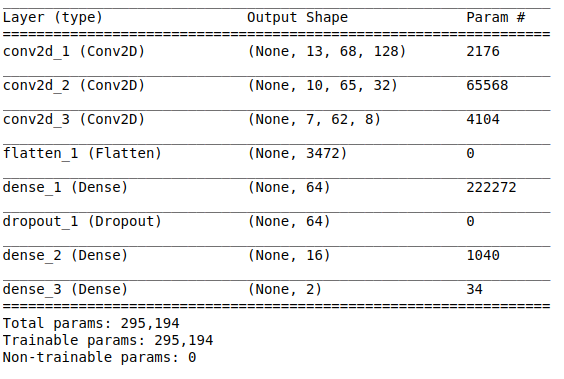
\includegraphics[width=\textwidth]{section3/modelparameters.png}
	\caption{
وزن‌های قابل یادگیری شبکه‌ی عصبی پیش‌بینی دوکلاسه}
	\label{paramNumber1}
\end{figure}

\newpage
در ساخت شبکه عصبی کانولوشن از تنظیمات زیر استفاده می‌شود:

۱) برای پیاده‌سازی شبکه عصبی از بسته‌های
\lr{Tensorflow}\cite{TENSORFLOW114}
(نسخه‌ی ۱.۱۴.۰) و
\lr{KERAS}\cite{KERAS2020}
(نسخه‌ی ۲.۲.۵) استفاده شد.

۲) از تابع بهینه‌سازی
\lr{ADAM}
استفاده شد.
 
۳) تابع خطا
\lr{Categorical-cross entropy}
در نظر گرفته شد.

۴) تعداد ایپوک
\LTRfootnote{Epoch}
ها ۵ در نظر گرفته شد. 

۵) نرخ یادگیری
\LTRfootnote{Lerning Rate}
۰/۰۰۰۰۱ استفاده شد.

درنظر داشته‌ باشید فراپارامترهای
\LTRfootnote{Hyperparameter}
این شبکه بهینه نشده ‌است و پارامترهای مشخص ‌شده لزوما در بهترین حالت خود نیستند. برای عدم بهینه‌سازی فراپارامترها دو دلیل وجود دارد:

۱) اجتناب از بیش‌برازش مدل
\LTRfootnote{Overfiting}:
در صورت تغییر فراپارامترها به بهترین مقادیر، انتظار می‌رود، مدل نتایج بهتری روی داده‌ی حاضر بگیرد، اما تضمینی وجود ندارد ویژگی‌های استخراج شده توسط مدل، معنی‌دار بوده و در صورت استفاده از مدل بر روی داروهای جدید به‌خوبی عمل کند. در این صورت اصطلاحا مدل بیش‌برازش شده و نکته‌ی منفی برای مدل خواهد بود. 

۲) حفظ استواری
\LTRfootnote{Robust}:
فراپارامترهای بهینه برای داده‌ی حاضر نتایج بهتری می‌دهند اما ممکن است در آینده از شباهت‌های دارویی متفاوتی استفاده شود یا داده‌های جدیدی جمع‌آوری شود و نتایج حاضر تکرار نشود. در این صورت مدل قوت و مستحکمی خود را از دست داده و مقبولیتی در جامعه‌ی داروسازی و داروشناسی نخواهد داشت.
 
 در نهایت نتایج مدل پیشنهادی را در روال اعتبارسنجی 10برابری از سه دیدگاه بررسی می کنیم:
 
 ۱) دقت مدل: مدل در روال اعتبارسنجی 10برابری برای تشخیص برهم‌کنش‌های کاهنده
$AUC=0/97$
و
$AUPR=0/93$ 
بدست آمد و برای تشخیص برهم‌کنش‌های افزاینده
$AUC=0/97$
و
$AUPR=0/99$
بدست آمد. این نتایج حاکی از دقت و توان تشخیص بالای مدل می‌باشد.
 
 ۲) واریانس نتایج: بازه‌ی اطمینان برای مقادیر گزارش‌شده با ضریب اطمینان بالای ۹۵ درصد باریک و نزدیک به‌هم بوده است. به شکلی که از چهار مقدار از سه مقدار گزارش شده کمتر از ۰/۰۰۲ بوده و  فقط برای تشخیص کاهنده مقدار 
\lr{AUPR}
 در بازه‌ی به اضافه و منهای ۰/۰۰۵ بوده‌است. با توجه به مقدار کم واریانس بدست آمده از مدل کاملا مشخص است که مدل ارایه شده استوار می‌باشد.
 

۳) توانایی تفکیک‌پذیری مدل: با رسم نمودار توزیع احتمالی خروجی ماشین مطابق شکل 
\ref{DDIProbHist}
 مشخص است که مقادیر 1 و 1- به‌خوبی از هم جدا شده‌اند و توزیع احتمال کاهنده و افزاینده اشترک کمی دارند. 


\begin{figure}[!h]
	\centering
	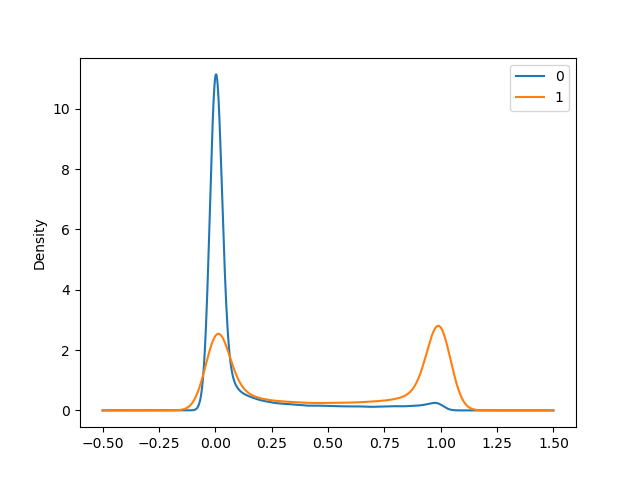
\includegraphics[scale=0.9]{section3/densityDegEnh.png}
	\caption{
نمودار توزیع چگالی احتمال کاهنده و افزاینده
}
در این شکل ۰ همان  برچسب ۱+ بوده و ۱ همان ۱- است.
	\label{DDIProbHist}
\end{figure}

شبه کد 
\ref{modelSelectionSuducode}
روند انتخاب مدل را مرحله به مرحله نشان می‌دهد.

\renewcommand{\algorithmicrequire}{\textbf{ورودی:}}
\renewcommand{\algorithmicensure}{\textbf{خروجی:}}
\begin{algorithm}[!h]
\caption{شبه کد انتخاب مدل}
\label{modelSelectionSuducode}
\begin{algorithmic}[1]
\REQUIRE 
ویژگی‌های جفت داروهای 1+ و 1-
\ENSURE 
مدل تشخیص دهنده 1+ و 1-
\vskip.5\baselineskip\hrule height 0.4pt\vskip.5\baselineskip

\STATE 
اعتبارسنجی متقابل 10 برابری را روی ویژگی‌های جفت داروهای 1+ و 1- اعمال کن.

\STATE 
مدل مناسب را انتخاب کن.

\STATE 
نتایج مدل را در روال اعتبارسنجی متقابل 10 برابری بررسی کن.

\STATE 
درصورت ارضای شرط ۳ مدل انتخابی را برگردان درغیراینصورت به مرحله ۲ بازگرد.

\end{algorithmic}
\end{algorithm}


\subsection{تشخیص جفت داروهای بدون برهم‌کنش احتمالی}

در مرحله‌ی قبل مدلی با دقت بالا، قوی و مستحکم ارائه شد که می‌توانست تاثیرات افزینده و کاهنده جفت داروها را به‌خوبی مدل کرده و تشخیص دهد. لذا این مدل به شرح زیر توانایی تشخیص غیربرهم‌کنش‌ها (صفرهای واقعی) را دارد. اگر با احتمال کمی جفت دارویی نامزد برهم‌کنش باشند، آنگاه آن جفت دارو، به احتمال زیاد، صفرهای واقعی هستند.

با توجه به این فرض، از مدل برای انجام پیش‌بینی روی کلیه‌ی جفت داروهای ناشناخته (صفرها) استفاده ‌شد. جفت داروهای ناشناخته شامل ۲۷۰۰۰۰ جفت دارو می‌باشد. در خروجی مدل، جفت داروهایی که با احتمال کمتر از ۰/۴ افزاینده و با احتمال کمتر از ۰/۴ کاهنده بودند را به  عنوان جفت داروهای بدون برهم‌کنش درنظر می‌گیریم. از بین داده‌هایی با برچسب ناشناخته حدود ۶۵۰۰۰ جفت دارو شرایط مذکور را داشتند. این دسته از جفت داروها نامزد عدم برهم‌کنش هستند. با توجه به دقت بالای مدل، واریانس کم نتایج و توانایی تفکیک‌پذیری بالای مدل، جفت‌های مذکور را به عنوان جفت داروهای فاقد برهم‌کنش در نظر می‌گیریم.

\subsection{آموزش مدل روی برهم‌کنش‌های شناخته‌شده و ناشناخته}

در این بخش از داده‌های شناخته شده و نامزدهای بالقوه برای عدم برهم‌کنش در جهت تشکیل مجموعه داده استفاده می‌شود. در این نگارش از این پس، جفت داروهای نامزد عدم برهم‌کنش را با عبارت صفر واقعی جایگزین کرده و به‌کار می‌بریم. همچنین برای مدل نهایی نیز از مدل توصیه‌گر ارائه‌شده در بخش
\ref{selected_model}
استفاده می‌شود. در ادامه روند کار به‌شکل مبسوط آمده است.

\subsubsection{روند اعتبارسنجی نتایج مدل پیش‌بینی برهم‌کنش داروها}
ابتدا سطرهایی از ماتریس
\lr{B}
که شامل برهم‌کنش‌‌‌های مثبت یک و منفی یک هستند مطابق روند مشروح در بخش
\ref{Model_selection_CV}
جدا شده و در 10 دسته قرار می‌گیرند. سپس به‌صورت تصادفی از میان ۶۵۰۰۰ جفت داروی نامزد بدون برهم‌کنش، ۳۰۰۰۰ جفت دارو انتخاب شد. در جفت داروی انتخابی، حتما باید خود جفت و دوگان آن نامزد بدون برهم‌کنش باشند. این گروه از صفرها به‌صورت تصادفی به ۱۰ دسته تقسیم می‌شوند. به‌گونه‌ای که دسته‌ی هر جفت دارو و دوگان یکسان باشد. سپس ۱۰ دسته‌ی صفرها با ۱۰ دسته‌ی از قبل آماده‌ی ۱+ و ۱- ها ادغام می‌شوند. 
 
حال مجموعه داده‌ای شامل تقریبا ۷۲۷۰۲ جفت دارو به دسته‌ی نسبتا برابر تقسیم شده و آماده‌ی استفاده برای روند آموزش و ارزیابی مدل نهایی توصیه‌گر می‌باشد.

\subsubsection{مدل نهایی پیش‌بینی برهم‌کنش داروها}

\begin{figure}
	\centering
	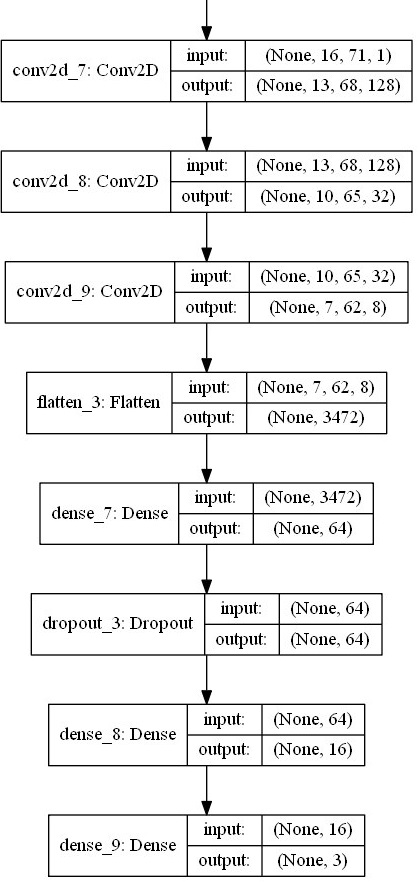
\includegraphics[scale=0.66]{section3/Triple_model.jpg}
	\caption{
چیدمان لایه‌های شبکه عصبی
\lr{SNF-CNN}
پیش‌بینی سه‌کلاسه برهم‌کنش
}
عدم برهم‌کنش (۰)، برهم‌کنش کاهنده (۱-) و برهم‌کنش افزاینده (۱+)
	\label{Triple_model}
\end{figure}
در قسمت قبل طریقه‌ی آماده‌سازی داده برای روال اعتبارسنجی مدل شرح داده‌شد. در این مرحله مدل نهایی ارائه می‌شود. مدل نهایی تقریبا همان مدل بیان شده در بخش 
\ref{selected_model}
است. یعنی شبکه سه لایه‌ی کانولوشن با تعداد فیلترهای کانولوشن ۱۲۸، ۳۲ و ۸ دارد. سپس همانند قبل از لایه‌های کانولوشن سه لایه تماما متصل استفاده شد. با این تفاوت که تعداد گره‌ها از ۶۴، ۱۶ و ۲  به ترتیب به ۶۴، ۱۶ و ۳ گره در هر لایه تغییر کرد. مشخصا این مدل سه خروجی احتمالی برای سه حالت برهم‌کنش افزاینده، عدم برهم‌کنش و برهم‌کنش کاهنده می‌دهد. همچنین تعداد ایپوک‌ها ۹ درنظر گرفته‌شد. روند انتخاب ایپوک در بخش
\ref{K-fold CV}
شرح داده ‌شده ‌است. مدل شبکه‌ی عصبی عمیق جهت پیش‌بینی برهم‌کنش در شکل
\ref{Triple_model}
نشان داده ‌شده ‌است. در این مرحله از انتخاب مدل جدید خودداری شد، زیرا:

۱) توان این مدل برای تشخیص نسبتا دقیق برهم‌کنش افزاینده و کاهنده در آخر بخش
\ref{selected_model}
به اثبات رسیده ‌است.

۲) صفرهای واقعی استفاده شده در این بخش پیشنهادی هستند و توسط آزمایشگاه داروشناسی تایید نشده‌اند و تا زمان نگارش این نوشتار پایگاه جامعی برای موارد عدم برهم‌کنش به‌صورت عمومی منتشر نشده ‌است. لذا اگر روند انتخاب مدل مجددا انجام شود، ممکن است مدلی انتخاب و استفاده شود که از نظر کاربرد در دنیای واقعی معتبر نبوده و مورد قبول قرار نگیرد.

با توجه به دلایل بالا مدل توصیه‌گر صفرها، با تغییر تعداد خروجی‌ها از ۲ به ۳ و تغییر داده‌های ورودی برای پیش‌برهم‌کنش‌های دارویی به‌کار می‌رود. فرآیند کلی روش پیشنهادی
\lr{SNF-CNN}
در قالب شبه کد 
\ref{SNFCNNSuducode}
ارائه شده است که شامل مراحل آماده‌سازی، انتخاب مدل، تشخیص صفر واقعی و ارائه‌ی توصیه‌گر جامع می‌باشد.

\renewcommand{\algorithmicrequire}{\textbf{ورودی:}}
\renewcommand{\algorithmicensure}{\textbf{خروجی:}}
\begin{algorithm}
\caption{
شبه کد روال کلی الگوریتم 
\lr{SNF-CNN}}
\label{SNFCNNSuducode}
\begin{algorithmic}[1]
\REQUIRE 
ویژگی‌های جفت داروها (1+، 1- و ۰های واقعی)
\ENSURE 
مدل تشخیص دهنده‌ی نوع برهم‌کنش و عدم‌برهم‌کنش (1+، 1- و ۰)
\vskip.5\baselineskip\hrule height 0.4pt\vskip.5\baselineskip

\STATE 
ماتریس‌های شباهت دارویی را با استفاده از روش کسینوس محاسبه کن.

\STATE 
ماتریس‌های شباهت دارویی را با استفاده از روش ترکیب شباهت شبکه‌ای ادغام کن.

\STATE 
ماتریس ورودی مدل را تشکیل بده.

\STATE 
مدل مناسب برهم‌کنش‌های شناخته شده را انتخاب کن و آموزش بده.

\STATE
صفرهای احتمالی را با استفاده از مرحله ۴ پیش‌بینی کن.
\STATE
مدل مناسب برهم‌کنش‌های شناخته شده و صفرهای مرحله ۵ را انتخاب کن و آموزش بده.
\STATE
روی جفت داروهای ناشناخته پیش‌بینی انجام بده.
\end{algorithmic}
\end{algorithm}


\section*{خلاصه‌ی فصل سوم و نگاهی به فصل چهار}
در این فصل روندی جامع برای آماده‌سازی داده ارائه ‌شد که می‌تواند بر روی ویژگی‌های مختلف اعمال شود و به انواع ماشین‌های یادگیرنده ورودی داده ‌شود. سپس مدل توصیه‌گری ارائه شد که نه تنها توانایی تشخیص نوع برهم‌کنش (افزاینده و کاهنده) را دارد بلکه می‌تواند جفت داروهایی را که به احتمال قوی باهم برهم‌کنش ندارند را نیز تشخیص دهد. روش ارائه شده به نام 
\lr{SNF-CNN}
نام‌گذاری شد. مدل توصیه‌گر سه‌کلاسه جامع در روند اعتبارسنجی آموزش و ارزیابی شد که نتایج آن در فصل چهار گزارش می‌شود. سپس برای اعتبارسنجی داروشناسی مدل با تمام جفت داروهای شناخته‌شده و صفرهای واقعی آموزش داده شد و روی تمام صفرها پیش‌بینی انجام شد و نتایج پیش‌بینی در پایگاه‌داده‌ی دارویی جست‌وجو شد که نتیجه اعتبارسنجی داروشناسی را نیز در فصل چهار ذکر شده و بررسی می‌شود.